\documentclass[9pt,a4paper]{extarticle}
\usepackage[a4paper,margin=1.4cm,top=1.2cm,bottom=1.3cm]{geometry}
\usepackage{fontspec}
\setmainfont{TeX Gyre Termes}
\setmonofont[Scale=0.85]{DejaVu Sans Mono}
\usepackage{unicode-math}
\setmathfont{Latin Modern Math}
\AtBeginDocument{\renewcommand{\figurename}{Figura}\renewcommand{\tablename}{Tabela}}
\usepackage{multicol,graphicx,booktabs,listings,xcolor,titlesec,enumitem,caption,float}
\usepackage[hidelinks]{hyperref}
\setlength{\columnsep}{0.55cm}
\titleformat{\section}{\normalfont\bfseries\normalsize}{\thesection}{0.5em}{}
\titleformat{\subsection}{\normalfont\bfseries\itshape\small}{\thesubsection}{0.5em}{}
\titlespacing*{\section}{0pt}{5pt}{2pt}
\titlespacing*{\subsection}{0pt}{3pt}{1pt}
\setlength{\parindent}{0pt}\setlength{\parskip}{2.5pt}
\setlist{nosep,leftmargin=1.1em}
\captionsetup{font=small,labelfont=bf,skip=2pt}
\pagestyle{plain}
\newcommand{\tl}{t_{\mathrm{local}}}
\lstset{basicstyle=\ttfamily\scriptsize,columns=fullflexible,keepspaces=true,breaklines=true,
  numbers=left,numberstyle=\tiny\color{gray},numbersep=4pt,frame=lines,framerule=0.3pt,
  commentstyle=\color[HTML]{5b6b7a}\itshape,keywordstyle=\color[HTML]{1c5cab}\bfseries,
  stringstyle=\color[HTML]{a3461c},showstringspaces=false,tabsize=4,aboveskip=4pt,belowskip=4pt}

\begin{document}
\begin{center}
{\large\bfseries T3 -- MPI com Fases Paralelas (FP): água presa no relevo do Rio Grande do Sul}\\[1pt]
{\small Marcelo A. F. Martins e Andriele B. Lange \quad|\quad Programação Paralela -- PUCRS \quad|\quad código: \texttt{github.com/MFelisberto/SimuChuvas}}
\end{center}
\vspace{-4pt}
\begin{multicols}{2}

\section{Problema}
Onde a chuva fica presa no RS? Usamos o relevo do estado inteiro (ANADEM, da ANA e do IPH/UFRGS: modelo de \emph{terreno} de 30\,m, sem o viés da vegetação), reamostrado para células de 60\,m: \textbf{12\,412 linhas $\times$ 14\,806 colunas = 184 milhões de células} (700\,MB). Para cada célula $c$ com altitude $Z(c)$ calculamos o nível $W(c)$ em que a água fica parada, pelo preenchimento de depressões de Planchon e Darboux. $W$ começa em $+\infty$ no interior e em $Z$ na borda do mapa e onde não há dado (mar, lagoas, países vizinhos), que funcionam como ralo. Depois, repete-se até nada mudar:
\[ W(c) \leftarrow \min\bigl(W(c),\ \max(Z(c),\ \min_{n} W(n))\bigr) \]
O termo $\min_n W(n)$ é o nível do vizinho $n$ mais baixo (8 vizinhos): a água de $c$ não precisa ficar acima dele, porque escoaria por ali. O $\max$ com $Z(c)$ garante que o nível nunca fica abaixo do chão, e o $\min$ externo, que o nível só desce. A profundidade é $W-Z$. Esse ponto fixo é único, então o resultado não depende da ordem de cálculo: \textbf{as 39 execuções deram o mesmo checksum} (\texttt{bb09d286e0336ace}): 7,34\,M células alagadas, até 210\,m de profundidade (cânion do Itaimbezinho). A opção \texttt{-L} impõe um nível nas bordas (ex.: 5,35\,m, o pico do Guaíba em maio de 2024) para as figuras de Porto Alegre do repositório.

\section{Modelo de fases paralelas}
O mapa é dividido em \textbf{faixas horizontais} de linhas, uma por processo (P0 = norte, P$_{p-1}$ = Chuí), cada uma com duas linhas fantasma (a borda dos vizinhos). O processo 0 lê o arquivo, calcula onde cada faixa começa (\texttt{MPI\_Bcast}) e distribui as faixas (\texttt{MPI\_Scatterv} com um tipo ``linha''). Depois, todos repetem:
\begin{enumerate}
\item \textbf{Processamento local:} até $k$ varreduras Gauss-Seidel na faixa, alternando 4 direções, só nas linhas marcadas como ``sujas''.
\item \textbf{Verificação distribuída:} \texttt{MPI\_Allreduce} (OU lógico) de ``minha faixa mudou?''. Se ninguém mudou, terminou.
\item \textbf{Troca com os vizinhos:} \texttt{MPI\_Sendrecv} da primeira e da última linha; se a fantasma recebida mudou, a linha de borda volta a ficar suja.
\end{enumerate}
O $k$ controla a granularidade da fase local (o análogo do \emph{chunk} do T1 e do $U$ do T2). Há duas divisões: \textbf{igual} (mesmo número de linhas) e \textbf{balanceada} (\texttt{-b}: mesmo número de células com dado, já que mar e Uruguai quase não custam).

\section{Metodologia}
Cluster \textbf{atlantica}, 4 nós exclusivos (Slurm), cada um com 2 soquetes $\times$ 4 núcleos e 2 \emph{threads} por núcleo (8 físicos, 16 lógicos), OpenMPI 4.1.1, \texttt{mpicc -O3}. Até 32 processos: $p/4$ por nó, um por núcleo físico (\texttt{--bind-to core}); com 64: 16 por nó, com HT (\texttt{--bind-to hwthread}). Ranks consecutivos ficam no mesmo nó, então só 3 fronteiras passam pela rede. A leitura do arquivo fica fora da medição. Cada configuração rodou 3 vezes e usamos o menor tempo (variação $<0{,}5\%$). A base é \texttt{mpirun -np 1} ($T_1 = 18{,}56$\,s, sem comunicação). Métricas: $S=T_1/T_p$ e $E=S/p$; \textbf{trabalho} = linhas visitadas $\div$ linhas do mapa (o sequencial varre o mapa o equivalente a 27,7 vezes), e eficiência de trabalho $=27{,}7/\text{trabalho}$; \textbf{desbal} = ($\tl$ máximo $-$ média)/média, como no T1/T2; $t_{\mathrm{verif}}$ inclui a espera pelo processo mais lento.

\section{Análise}
\subsection{Escalabilidade}
Com divisão balanceada e $k=2$, o speedup foi 2,9 / 4,5 / 6,3 / \textbf{10,5} com 4 / 8 / 16 / 32 processos (Tab.~1, Fig.~1). A comunicação não é o problema: a troca de bordas custa 0,06\,s (3\%). Com 32 processos, o tempo ideal seria 0,58\,s; chegamos a 1,77\,s por três motivos (Fig.~2):
\begin{itemize}
\item \textbf{Trabalho extra} ($\times1{,}35$): cada faixa começa sem conhecer a borda dos vizinhos e forma ``lagos falsos'' encostados nelas, que precisam ser esvaziados depois. Mais faixas, mais fronteiras.
\item \textbf{Custo por linha} (+13\%): 8 processos por nó dividem a banda de memória (54\,$\mu$s por linha com 1 processo, 61\,$\mu$s com 32).
\item \textbf{Espera} (0,82\,s, quase metade do tempo): a cada rodada, todos esperam o mais lento no \texttt{Allreduce}.
\end{itemize}

\subsection{Granularidade da fase local ($k$)}
Deixar cada faixa estabilizar sozinha ($k=\infty$) foi o pior caso: 5,70\,s com só 17 rodadas, mas trabalho 77 (2,8 vezes o sequencial), porque cada faixa resolve por inteiro um problema errado (os lagos falsos) antes de ouvir os vizinhos. Com $k$ pequeno a informação atravessa as fronteiras logo: $k=2$ foi o melhor (1,77\,s, 42 rodadas). Com $k=1$ as rodadas dobram (83) e a troca dobra (0,11\,s), e o tempo sobe um pouco (Fig.~3, Tab.~3).

\subsection{Balanceamento}
Na divisão igual, as faixas do norte (Alto Uruguai e Planalto, relevo recortado e cheio de depressões) levam até 1,58\,s, e as do sul (Campanha, Lagoa dos Patos) 0,37\,s: desbal = 78\%. A divisão balanceada baixou o desbal para 52\% e o maior $\tl$ em 14\%, mas \textbf{o tempo total não mudou} (1,77 contra 1,74\,s; Fig.~4, Tab.~2). Em FP, cada rodada espera o processo mais lento \emph{daquela rodada}, então o tempo é a soma dos máximos de cada rodada, e não o máximo das somas. A carga de cada rodada depende de onde está a frente de escoamento, que muda de faixa a faixa; dividir pela carga total não acompanha isso.

\subsection{Hyper-threading (64 processos)}
Com HT, o tempo piorou (1,96 contra 1,77\,s). Duas \emph{threads} no mesmo núcleo dividem o núcleo e a memória: o custo por linha quase dobra (61 para 113\,$\mu$s). Além disso, o dobro de faixas dá +24\% de trabalho e 52 rodadas em vez de 42. No T1/T2 o HT ajudou (+47\%), porque o cálculo era limitado pelo processador; aqui o \emph{stencil} é limitado pela memória.

\subsection{Conclusão}
O modelo FP se encaixa no problema (uma relaxação que converge por rodadas) e chegou a speedup 10,5 com 32 processos, com o mesmo resultado bit a bit em qualquer configuração. O que limita não é o volume de comunicação, e sim a sincronização a cada rodada e o trabalho extra criado pelas fronteiras entre faixas; por isso o melhor ajuste foi no $k$, e não na divisão das faixas.

\section{Declaração de uso de IA}
Usamos o Claude (Anthropic) para discutir a escolha do problema, escrever e revisar partes do código C e dos scripts em Python (preparação do mapa, figuras e animações), montar o script de execução no cluster e redigir este relatório. As execuções na atlantica foram feitas por nós, e revisamos o código e as conclusões.
\end{multicols}

\newpage
\section*{Gráficos e tabelas}
\begin{figure}[H]\centering
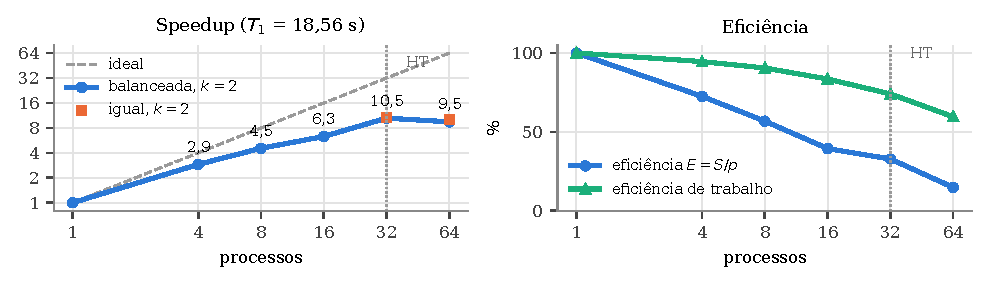
\includegraphics[width=\linewidth]{fig/speedup.pdf}
\caption{Speedup e eficiência (escalas log$_2$). A linha pontilhada em 32 marca o fim dos núcleos físicos; à direita, HT. Eficiência de trabalho = trabalho do sequencial / trabalho paralelo.}
\end{figure}
\vspace{-6pt}
\begin{figure}[H]\centering
\begin{minipage}{0.49\linewidth}\centering
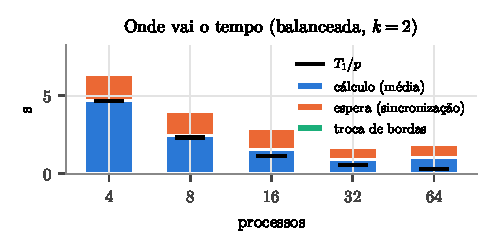
\includegraphics[width=\linewidth]{fig/tempo.pdf}
\caption{Divisão do tempo total: cálculo médio por processo, espera no \texttt{Allreduce} e troca de bordas. O traço preto é o ideal $T_1/p$.}
\end{minipage}\hfill
\begin{minipage}{0.49\linewidth}\centering
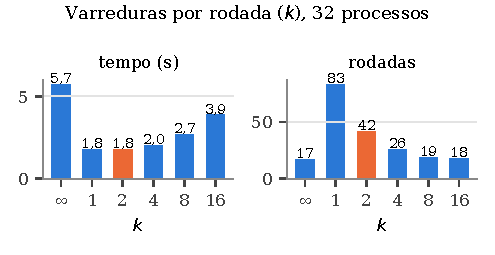
\includegraphics[width=\linewidth]{fig/k.pdf}
\caption{Efeito de $k$ (varreduras por rodada) com 32 processos; $\infty$ = cada faixa estabiliza antes de trocar. Em laranja, o $k$ usado.}
\end{minipage}
\end{figure}
\vspace{-6pt}
\begin{figure}[H]\centering
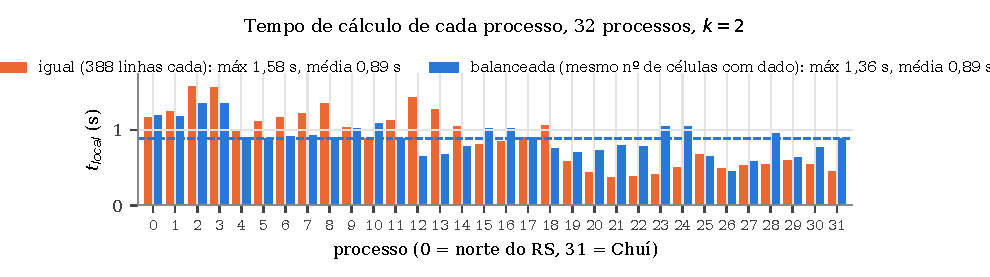
\includegraphics[width=\linewidth]{fig/carga.pdf}
\caption{Tempo de cálculo ($\tl$) de cada processo, divisão igual e balanceada (32 processos, $k=2$); tracejado = média. Na balanceada as faixas do sul (26--31) ficam com 2 a 3 vezes mais linhas, porque metade delas é mar.}
\end{figure}

\begin{minipage}[t]{0.56\linewidth}
\captionof{table}{Escalabilidade (divisão balanceada, $k=2$; melhor de 3).}
\centering\small\setlength{\tabcolsep}{3.5pt}
\begin{tabular}{rrrrrrrrr}\toprule
$p$ & $T_p$ (s) & $S$ & $E$ & rodadas & trabalho & $t_{\mathrm{verif}}$ & $t_{\mathrm{troca}}$ & desbal\\\midrule
1  & 18,560 & 1,00  & 100\% & 2  & 27,7 & -- & -- & -- \\
4  & 6,399  & 2,90  & 73\%  & 42 & 29,3 & 1,99 & 0,073 & 16\% \\
8  & 4,085  & 4,54  & 57\%  & 42 & 30,6 & 1,97 & 0,069 & 34\% \\
16 & 2,943  & 6,31  & 39\%  & 42 & 33,2 & 1,95 & 0,062 & 54\% \\
32 & \textbf{1,768} & \textbf{10,50} & 33\% & 42 & 37,4 & 1,31 & 0,056 & 52\% \\
64 (HT) & 1,961 & 9,46 & 15\% & 52 & 46,5 & 1,49 & 0,079 & 47\% \\\bottomrule
\end{tabular}
\end{minipage}\hfill
\begin{minipage}[t]{0.42\linewidth}
\captionof{table}{Divisão das faixas ($k=2$).}
\centering\small\setlength{\tabcolsep}{3.5pt}
\begin{tabular}{rlrrrr}\toprule
$p$ & divisão & $T_p$ (s) & $\tl$ máx & desbal & rod.\\\midrule
32 & igual      & 1,738 & 1,58 & 78\% & 42\\
32 & balanceada & 1,768 & 1,35 & 52\% & 42\\
64 & igual      & 1,824 & 1,66 & 67\% & 46\\
64 & balanceada & 1,961 & 1,50 & 47\% & 52\\\bottomrule
\end{tabular}

\vspace{6pt}
\captionof{table}{Efeito de $k$ (32 processos, balanceada).}
\setlength{\tabcolsep}{3.5pt}
\begin{tabular}{lrrrrrr}\toprule
$k$ & $\infty$ & 1 & 2 & 4 & 8 & 16\\\midrule
$T_p$ (s) & 5,70 & 1,79 & \textbf{1,77} & 2,00 & 2,69 & 3,87\\
rodadas & 17 & 83 & 42 & 26 & 19 & 18\\
trabalho & 77,1 & 37,4 & 37,4 & 44,6 & 58,3 & 71,7\\
$t_{\mathrm{verif}}$ (s) & 4,93 & 1,32 & 1,31 & 1,47 & 1,95 & 3,10\\\bottomrule
\end{tabular}
\end{minipage}

\newpage
\section*{Código-fonte}
Compilação: \texttt{make mpi}; mapa: \texttt{make dados} (remonta \texttt{dados/rs.dem} a partir das partes do repositório). Execução: \texttt{mpirun -np 32 ./mpi -b -k 2 dados/rs.dem}. Bateria completa: \texttt{sbatch run\_grid.sh}.
\lstinputlisting[language=C,title={\small\texttt{src/mpi.c}}]{../src/mpi.c}
\lstinputlisting[language=C,title={\small\texttt{src/common.h}}]{../src/common.h}
\lstinputlisting[language=C,title={\small\texttt{src/common.c}}]{../src/common.c}
\lstinputlisting[language=bash,title={\small\texttt{run\_grid.sh}}]{../run_grid.sh}
\end{document}
